% Options for packages loaded elsewhere
% Options for packages loaded elsewhere
\PassOptionsToPackage{unicode}{hyperref}
\PassOptionsToPackage{hyphens}{url}
%
\documentclass[
  12pt,
  letterpaper,
  DIV=11,
  numbers=noendperiod]{scrartcl}
\usepackage{xcolor}
\usepackage[left=1in,right=1in,top=1in,bottom=1in]{geometry}
\usepackage{amsmath,amssymb}
\setcounter{secnumdepth}{5}
\usepackage{iftex}
\ifPDFTeX
  \usepackage[T1]{fontenc}
  \usepackage[utf8]{inputenc}
  \usepackage{textcomp} % provide euro and other symbols
\else % if luatex or xetex
  \usepackage{unicode-math} % this also loads fontspec
  \defaultfontfeatures{Scale=MatchLowercase}
  \defaultfontfeatures[\rmfamily]{Ligatures=TeX,Scale=1}
\fi
\usepackage{lmodern}
\ifPDFTeX\else
  % xetex/luatex font selection
  \setmainfont[ItalicFont=EB Garamond Italic,BoldFont=EB Garamond
SemiBold]{EB Garamond Math}
  \setsansfont[]{EB Garamond SemiBold}
  \setmathfont[]{EB Garamond Math}
\fi
% Use upquote if available, for straight quotes in verbatim environments
\IfFileExists{upquote.sty}{\usepackage{upquote}}{}
\IfFileExists{microtype.sty}{% use microtype if available
  \usepackage[]{microtype}
  \UseMicrotypeSet[protrusion]{basicmath} % disable protrusion for tt fonts
}{}
\usepackage{setspace}
% Make \paragraph and \subparagraph free-standing
\makeatletter
\ifx\paragraph\undefined\else
  \let\oldparagraph\paragraph
  \renewcommand{\paragraph}{
    \@ifstar
      \xxxParagraphStar
      \xxxParagraphNoStar
  }
  \newcommand{\xxxParagraphStar}[1]{\oldparagraph*{#1}\mbox{}}
  \newcommand{\xxxParagraphNoStar}[1]{\oldparagraph{#1}\mbox{}}
\fi
\ifx\subparagraph\undefined\else
  \let\oldsubparagraph\subparagraph
  \renewcommand{\subparagraph}{
    \@ifstar
      \xxxSubParagraphStar
      \xxxSubParagraphNoStar
  }
  \newcommand{\xxxSubParagraphStar}[1]{\oldsubparagraph*{#1}\mbox{}}
  \newcommand{\xxxSubParagraphNoStar}[1]{\oldsubparagraph{#1}\mbox{}}
\fi
\makeatother


\usepackage{longtable,booktabs,array}
\usepackage{calc} % for calculating minipage widths
% Correct order of tables after \paragraph or \subparagraph
\usepackage{etoolbox}
\makeatletter
\patchcmd\longtable{\par}{\if@noskipsec\mbox{}\fi\par}{}{}
\makeatother
% Allow footnotes in longtable head/foot
\IfFileExists{footnotehyper.sty}{\usepackage{footnotehyper}}{\usepackage{footnote}}
\makesavenoteenv{longtable}
\usepackage{graphicx}
\makeatletter
\newsavebox\pandoc@box
\newcommand*\pandocbounded[1]{% scales image to fit in text height/width
  \sbox\pandoc@box{#1}%
  \Gscale@div\@tempa{\textheight}{\dimexpr\ht\pandoc@box+\dp\pandoc@box\relax}%
  \Gscale@div\@tempb{\linewidth}{\wd\pandoc@box}%
  \ifdim\@tempb\p@<\@tempa\p@\let\@tempa\@tempb\fi% select the smaller of both
  \ifdim\@tempa\p@<\p@\scalebox{\@tempa}{\usebox\pandoc@box}%
  \else\usebox{\pandoc@box}%
  \fi%
}
% Set default figure placement to htbp
\def\fps@figure{htbp}
\makeatother


% definitions for citeproc citations
\NewDocumentCommand\citeproctext{}{}
\NewDocumentCommand\citeproc{mm}{%
  \begingroup\def\citeproctext{#2}\cite{#1}\endgroup}
\makeatletter
 % allow citations to break across lines
 \let\@cite@ofmt\@firstofone
 % avoid brackets around text for \cite:
 \def\@biblabel#1{}
 \def\@cite#1#2{{#1\if@tempswa , #2\fi}}
\makeatother
\newlength{\cslhangindent}
\setlength{\cslhangindent}{1.5em}
\newlength{\csllabelwidth}
\setlength{\csllabelwidth}{3em}
\newenvironment{CSLReferences}[2] % #1 hanging-indent, #2 entry-spacing
 {\begin{list}{}{%
  \setlength{\itemindent}{0pt}
  \setlength{\leftmargin}{0pt}
  \setlength{\parsep}{0pt}
  % turn on hanging indent if param 1 is 1
  \ifodd #1
   \setlength{\leftmargin}{\cslhangindent}
   \setlength{\itemindent}{-1\cslhangindent}
  \fi
  % set entry spacing
  \setlength{\itemsep}{#2\baselineskip}}}
 {\end{list}}
\usepackage{calc}
\newcommand{\CSLBlock}[1]{\hfill\break\parbox[t]{\linewidth}{\strut\ignorespaces#1\strut}}
\newcommand{\CSLLeftMargin}[1]{\parbox[t]{\csllabelwidth}{\strut#1\strut}}
\newcommand{\CSLRightInline}[1]{\parbox[t]{\linewidth - \csllabelwidth}{\strut#1\strut}}
\newcommand{\CSLIndent}[1]{\hspace{\cslhangindent}#1}



\setlength{\emergencystretch}{3em} % prevent overfull lines

\providecommand{\tightlist}{%
  \setlength{\itemsep}{0pt}\setlength{\parskip}{0pt}}



 


\setlength\heavyrulewidth{0ex}
\setlength\lightrulewidth{0ex}
\KOMAoption{captions}{tableheading}
\makeatletter
\@ifpackageloaded{caption}{}{\usepackage{caption}}
\AtBeginDocument{%
\ifdefined\contentsname
  \renewcommand*\contentsname{Table of contents}
\else
  \newcommand\contentsname{Table of contents}
\fi
\ifdefined\listfigurename
  \renewcommand*\listfigurename{List of Figures}
\else
  \newcommand\listfigurename{List of Figures}
\fi
\ifdefined\listtablename
  \renewcommand*\listtablename{List of Tables}
\else
  \newcommand\listtablename{List of Tables}
\fi
\ifdefined\figurename
  \renewcommand*\figurename{Figure}
\else
  \newcommand\figurename{Figure}
\fi
\ifdefined\tablename
  \renewcommand*\tablename{Table}
\else
  \newcommand\tablename{Table}
\fi
}
\@ifpackageloaded{float}{}{\usepackage{float}}
\floatstyle{ruled}
\@ifundefined{c@chapter}{\newfloat{codelisting}{h}{lop}}{\newfloat{codelisting}{h}{lop}[chapter]}
\floatname{codelisting}{Listing}
\newcommand*\listoflistings{\listof{codelisting}{List of Listings}}
\makeatother
\makeatletter
\makeatother
\makeatletter
\@ifpackageloaded{caption}{}{\usepackage{caption}}
\@ifpackageloaded{subcaption}{}{\usepackage{subcaption}}
\makeatother
\usepackage{bookmark}
\IfFileExists{xurl.sty}{\usepackage{xurl}}{} % add URL line breaks if available
\urlstyle{same}
\hypersetup{
  pdftitle={When are Philosophy Articles Cited?},
  pdfauthor={Anon},
  hidelinks,
  pdfcreator={LaTeX via pandoc}}


\title{When are Philosophy Articles Cited?}
\author{Anon}
\date{2025-06-14}
\begin{document}
\maketitle
\begin{abstract}
It's natural to believe that philosophy citations are typically to long
ago pieces. We're still talking about philosophers from millenia ago.
More strikingly, we're still talking about papers from half a century
ago not as historical papers, but as part of the contemporary debate.
But a systematic look at the citation data shows that these cases are
outliers. Most citations are to recently published works. Surprisingly,
this is less true in recent years than it used to be. The effect of
electronic publishing and communication has been to make citations, on
average, older. After we adjust for the typical age of philosophy
citations, and this changing trend, it turns out that the 2000s were a
particularly influential time in philosophy publishing. Articles
published in that decade are cited more than earlier or later articles,
once we adjust for the typical times articles are cited, and the
changing patterns of citation. This is arguably related to broad changes
in the interests of philosophers, towards social philosophy, and
epistemology.
\end{abstract}


\setstretch{1.75}
\section{Introduction}\label{sec-introduction}

This paper is about the patterns of citations of philosophy journal
articles in philosophy journals. Obviously philosophy journals cite more
things than philosophy journals, and just as obviously philosophy
journal articles get cited in other places. But looking just at
journal-to-journal citations allows us to get a citation set that is
relatively complete, and hence make some systematic generalisations
about the way articles are cited over time. It turns out some of these
generalisations are surprising.

Before looking at the data, here are two things I believed about
philosophy citations. First, philosophers tend to cite very old papers.
We still regularly teach a number of papers over half a century old in
introductory classes; e.g., Frankfurt
(\citeproc{ref-WOSA1969Y444700002}{1969}), Thomson
(\citeproc{ref-WOSA1971Y116900003}{1971}), Singer
(\citeproc{ref-WOSA1972Z066400001}{1972}), and Lewis
(\citeproc{ref-10.2307_2025310}{1973}). These aren't taught as history
papers, but as early entries into the contemporary philosophical debate.
While most papers aren't cited as much as these papers are, I thought
the pattern that old papers keep being cited extended to their less
famous counterparts. Second, the technological changes of the last
quarter century meant that this practice was being slowly reversed. A
series of technological innovations made it easier to cite newer and
newer works. These innovations included the spread of email, the rise of
preprint archives (e.g., arXiv, SSRN, PhilPapers), and eventually
official preprints in things like EarlyView. So, I thought, citations
should be getting younger, because the delay between publishing and
getting widely known was removed.

Both of these thoughts were wrong.

On the first point, the generalisation I made from those famous papers
was just wrong. Normal papers differ from famous papers not just in how
often they are cited, but in the shape of their citations. The main
evidence I'll use for this is something I'll call the \emph{citation
ratio}. The citation ratio of year \emph{o} in year \emph{n} is the mean
number of citations, in year \emph{n}, of articles published in year
\emph{o}, divided by the mean number of citations, in year \emph{n}, of
articles published in years \emph{n}-10 to \emph{n}-3. (I'll say much
more about why I'm using this measure in what follows.)
Figure~\ref{fig-master-citation-ratio} shows the average citation ratio
for different \emph{ages}, of citations, i.e., the number of years
between \emph{o} and \emph{n}.\footnote{The graph also includes some
  `jitter' to make the different points more easily visible. I've put
  each decade of original publication in a different colour; I'll break
  those out in Figure~\ref{fig-decades-cite-ratio}. The graph starts in
  1975 because the data is much noisier before then, for reasons we'll
  get to below.}

\begin{figure}

\centering{

\pandocbounded{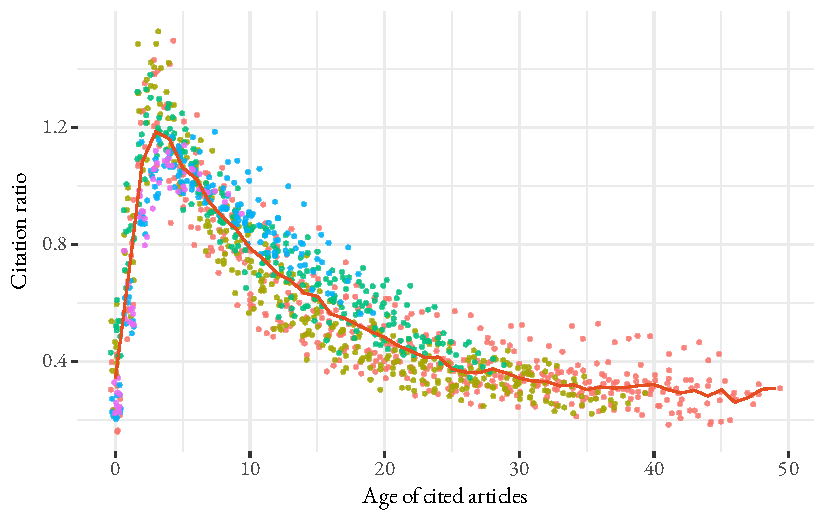
\includegraphics[keepaspectratio]{apc-2025-june-draft_files/figure-pdf/fig-master-citation-ratio-1.pdf}}

}

\caption{\label{fig-master-citation-ratio}Age effects from 1975 onwards
on a single graph, with the overall average shown.}

\end{figure}%

Each dot on that graph is a citation ratio for a particular pair of
years; the line shows the average citation ratio for all pairs with the
same age. The shape is unmistakable; articles get cited much much more
when they are relatively young than when they are older.

The `evidence' I gave for the opposite view in the introductory
paragraph wasn't entirely wrong. If we redo
Figure~\ref{fig-master-citation-ratio} just looking at articles which
have 15 or more citations in philosophy journals. (This turns out to be
a fairly small percentage of the sample.)

\begin{figure}

\centering{

\pandocbounded{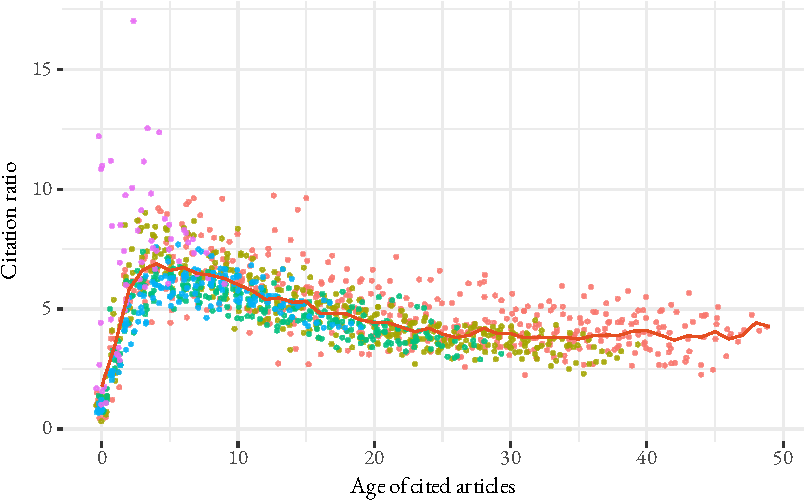
\includegraphics[keepaspectratio]{apc-2025-june-draft_files/figure-pdf/fig-ageeffecteverything-high-1.pdf}}

}

\caption{\label{fig-ageeffecteverything-high}A version of
Figure~\ref{fig-master-citation-ratio} just looking at highly cited
articles}

\end{figure}%

The numbers on the y-axis in Figure~\ref{fig-ageeffecteverything-high}
are higher than in Figure~\ref{fig-master-citation-ratio}. That's not
surprising; it just means highly cited articles get cited more
frequently. What is striking is the different shape of the graphs.
Typical philosophy articles, if they get cited at all, get cited soon
after publication and they fade into obscurity. Highly cited articles
keep getting cited decades after their publication.

These results aren't a priori obvious; things could have turned out
otherwise. It could have been that there were a trove of articles which
were ignored after publication and then accrued five to ten citations a
couple of decades later. There are some articles that were very
frequently cited soon after publication but which are now largely
ignored. (This happens most frequently in philosophy of science and in
philosophy of mind, I think for different reasons in the two cases.) But
these cases are outliers. Most of the articles that were influential
soon after publication stay that way.

For the second point, we can simply break up
Figure~\ref{fig-master-citation-ratio} by ten year chunks. In
Figure~\ref{fig-decades-cite-ratio} I've taken the points by from
Figure~\ref{fig-master-citation-ratio}, and grouped them into `decades'.
Because I'm working here with 1975-2024 data, the decades are 1975-1984,
1985-1994 etc. To make it easier to compare decades, I've removed the
last one, where there isn't enough data, and removed all points with an
age over 20.

\begin{figure}

\begin{minipage}{0.50\linewidth}

\centering{

\pandocbounded{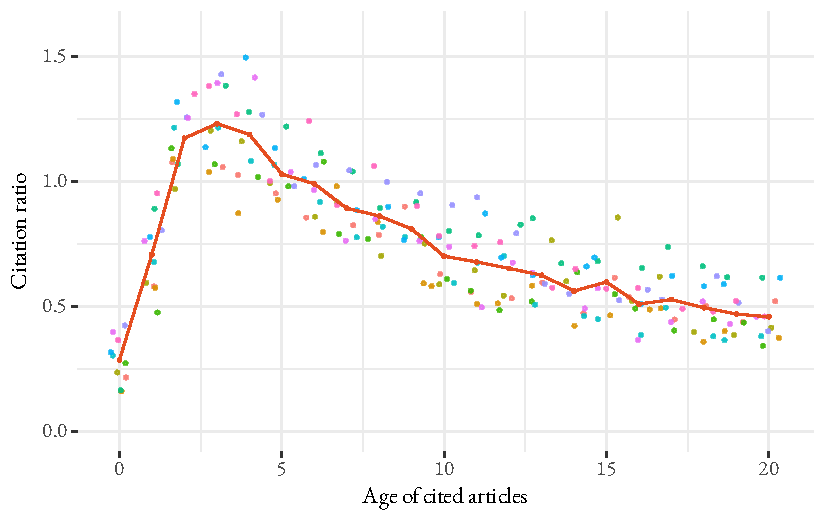
\includegraphics[keepaspectratio]{apc-2025-june-draft_files/figure-pdf/fig-decades-cite-ratio-1.pdf}}

}

\subcaption{\label{fig-decades-cite-ratio-1}1975-1984}

\end{minipage}%
%
\begin{minipage}{0.50\linewidth}

\centering{

\pandocbounded{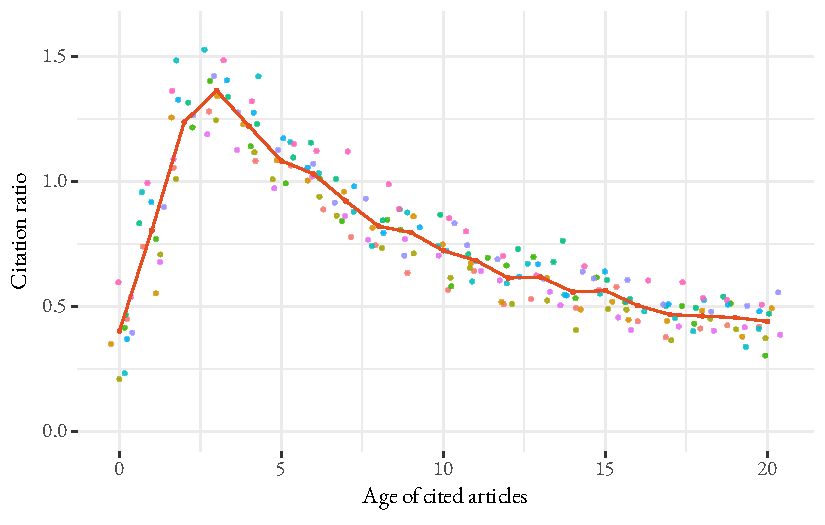
\includegraphics[keepaspectratio]{apc-2025-june-draft_files/figure-pdf/fig-decades-cite-ratio-2.pdf}}

}

\subcaption{\label{fig-decades-cite-ratio-2}1985-1994}

\end{minipage}%
\newline
\begin{minipage}{0.50\linewidth}

\centering{

\pandocbounded{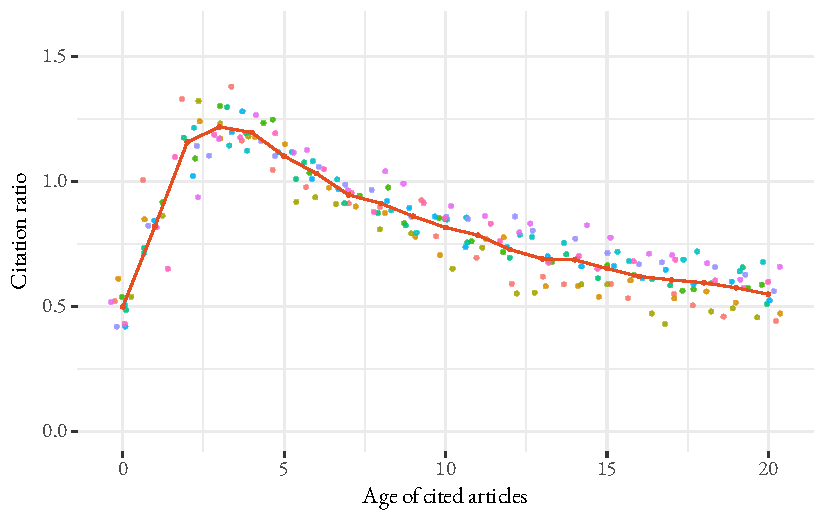
\includegraphics[keepaspectratio]{apc-2025-june-draft_files/figure-pdf/fig-decades-cite-ratio-3.pdf}}

}

\subcaption{\label{fig-decades-cite-ratio-3}1995-2004}

\end{minipage}%
%
\begin{minipage}{0.50\linewidth}

\centering{

\pandocbounded{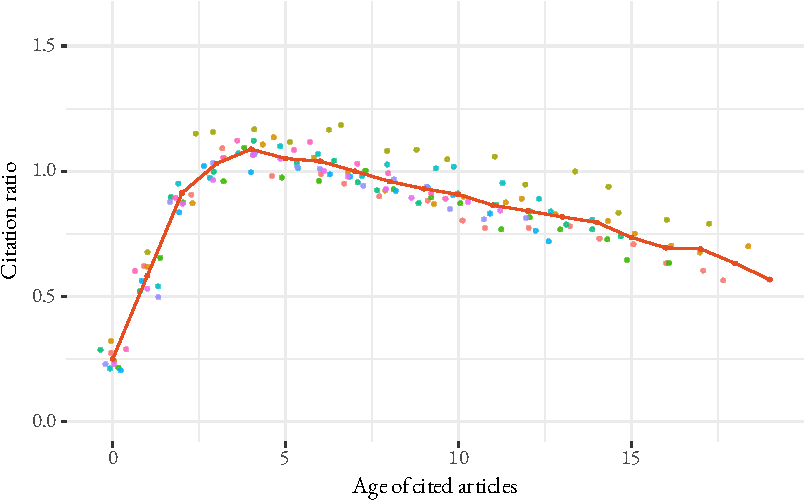
\includegraphics[keepaspectratio]{apc-2025-june-draft_files/figure-pdf/fig-decades-cite-ratio-4.pdf}}

}

\subcaption{\label{fig-decades-cite-ratio-4}2005-2014}

\end{minipage}%

\caption{\label{fig-decades-cite-ratio}Citation ratio for different
decades}

\end{figure}%

\phantomsection\label{refs}
\begin{CSLReferences}{1}{0}
\bibitem[\citeproctext]{ref-WOSA1969Y444700002}
Frankfurt, Harry G. 1969. {``Alternate Possibilities and Moral
Responsibility.''} \emph{Journal of Philosophy} 66 (23): 829--39.
\url{https://doi.org/10.2307/2023833}.

\bibitem[\citeproctext]{ref-10.2307_2025310}
Lewis, David. 1973. {``Causation.''} \emph{Journal of Philosophy} 70
(17): 556--67.

\bibitem[\citeproctext]{ref-WOSA1972Z066400001}
Singer, Peter. 1972. {``Famine, Affluence, and Morality.''}
\emph{Philosophy \& Public Affairs} 1 (3): 229--43.

\bibitem[\citeproctext]{ref-WOSA1971Y116900003}
Thomson, Judith Jarvis. 1971. {``A Defense of Abortion.''}
\emph{Philosophy \& Public Affairs} 1 (1): 47--66.

\end{CSLReferences}




\end{document}
